% ----------------------------------------------------------
% ESCOPO
% ----------------------------------------------------------
\section{Escopo}

Neste tópico são abordados os casos de uso da aplicação (forma de descrever uma funcionalidade do sistema); diagrama de requisitos (identificação das funcionalidades a serem implementadas); histórias de usuário (descrição das necessidades do usuário); e definição de entregas (quais funcionalidades estarão disponíveis nas principais entregas).
% ----------------------------------------------------------
% REQUISITOS
% ----------------------------------------------------------
\subsection{Requisitos}

Para o desenvolvimento da aplicação \emph{EstagiEI}, são expostos os requisitos funcionais, não-funcionais e regras de negócio que a aplicação terá, tais requisitos foram formados a partir de estudos de como irão funcionar os processos do sistema em construção.

% ----------------------------------------------------------
% REQUISITOS FUNCIONAIS
% ----------------------------------------------------------
\subsubsection{Requisitos Funcionais}

Os requisitos funcionais dizem respeito às principais funcionalidades que o sistema deve empenhar \cite{sommerville}. Durante nossa análise, foram decididos os principais requisitos funcionais da aplicação como descrito no \autoref{req-fun}:

\begin{quadro}[H]
\ABNTEXfontereduzida
\centering
\caption[Requisitos funcionais]{Requisitos funcionais}
    \begin{tabular}{|l|l|}
    \hline
    \multicolumn{1}{|c|}{\textbf{Código}} &
      \multicolumn{1}{c|}{\textbf{Descrição}} \\ \hline
    RF-001 &
      \begin{tabular}[c]{@{}l@{}}Permitir a busca de vagas por filtros\end{tabular} \\ \hline
    RF-002 &
      \begin{tabular}[c]{@{}l@{}}Recomendar vagas para estudantes, empresas para estudantes, estudantes \\ para vagas/empresas\end{tabular} \\ \hline
    RF-003 &
      Manter um histórico de vagas tanto para o candidato, quanto para a empresa \\ \hline
    RF-004 &
      Exibir uma linha do tempo do andamento da vaga \\ \hline
    RF-005 &
      Alertar os estudantes aplicados à vaga sobre cada mudança em seu processo \\ \hline
    RF-006 &
      \begin{tabular}[c]{@{}l@{}}Possibilitar que a empresa possa entrar em contato com os estudantes \\ recomendados/aplicados à vaga\end{tabular} \\ \hline
    RF-007 &
      Possibilitar que a empresa realize mudanças no status de andamento da vaga \\ \hline
    RF-008 &
      \begin{tabular}[c]{@{}l@{}}Possibilitar que o estudante realize um \textit{feedback} da empresa pós-entrevista, \\ que será visto por outros estudantes\end{tabular} \\ \hline
    RF-009 &
      \begin{tabular}[c]{@{}l@{}}Não permitir o registro de vagas cujas horas de atividades ultrapassem \\ a carga horária prevista por lei de acordo com a situação escolar de cada estudante\end{tabular} \\ \hline
    RF-010 &
    \begin{tabular}[c]{@{}l@{}}Permitir o cadastro de vagas por parte da empresa, seguindo as regras estabelecidas\end{tabular} \\ \hline
    \end{tabular}
    \fonte{Os Autores}
    \label{req-fun}
\end{quadro}

% ----------------------------------------------------------
% REQUISITOS NÃO-FUNCIONAIS
% ----------------------------------------------------------
\subsubsection{Requisitos Não-funcionais}

Ao contrário dos requisitos funcionais, os requisitos não-funcionais não estão ligados às principais funcionalidades de um sistema, mas sim com seus fatores de restrições e especificações. É a partir deles que são observados aspectos como desempenho, usabilidade, segurança e outros aspectos não-funcionais que tangem o sistema \cite{sommerville}.
Tendo isto em mente, no \autoref{req-nao-fun} são elencados os principais requisitos não-funcionais. 
\begin{quadro}[H]
\centering
\ABNTEXfontereduzida
\caption[Requisitos não funcionais]{Requisitos não-funcionais}
    \begin{tabular}{|l|l|}
    \hline
    \multicolumn{1}{|c|}{\textbf{Código}} & \multicolumn{1}{c|}{\textbf{Descrição}}                                 \\ \hline
    RNF-001                               & O sistema deve oferecer boa usabilidade (Ser fácil de aprender a usar)  \\ \hline
    RNF-002                               & O sistema deve estar disponível 24 horas por dia, 7 dias por semana     \\ \hline
    RNF-003                               & O sistema deve possuir possibilidade de escalabilidade                  \\ \hline
    RNF-004                               & Tempo para o carregamento que satisfaça as expectativas do cliente      \\ \hline
    RNF-005                               & O sistema deve possuir uma taxa de ocorrência de falhas menor que 0.3\% \\ \hline
    RNF-006                               & O sistema deve estar de acordo com a \ac{lgpd}                          \\ \hline
    RNF-007 & \begin{tabular}[c]{@{}l@{}}O sistema deve estar de acordo com a lei Nº 11.788, de 25 de setembro de 2008, \\ regulando a carga horária do estágio\end{tabular} \\ \hline
    RNF-008 & \begin{tabular}[c]{@{}l@{}}O sistema deve ser responsivo aos diferentes dispositivos que os usuários \\ podem utilizar para acessá-lo\end{tabular}             \\ \hline
    \end{tabular}
    \fonte{Os Autores}
    \label{req-nao-fun}
\end{quadro}

% ----------------------------------------------------------
% REGRAS DE NEGÓCIO
% ----------------------------------------------------------
\subsubsection{Regras de Negócio}
As regras de negócio, que estão ligadas aos requisitos funcionais previamente descritos, do nosso projeto estão listados no \autoref{regra-negocio}.

\begin{quadro}[H]
\centering
\ABNTEXfontereduzida
\caption[Regras de negócio]{Regras de negócio}
    \begin{tabular}{|l|l|l|}
    \hline
    \multicolumn{1}{|c|}{\textbf{Código}} &
      \multicolumn{1}{c|}{\textbf{Descrição}} &
      \multicolumn{1}{c|}{\textbf{Requisito Relacionado}} \\ \hline
    RN-001 &
      \begin{tabular}[c]{@{}l@{}}As vagas a serem cadastradas devem estar \\ coerentes com o perfil buscado\end{tabular} &
      RF-010 \\ \hline
    RN-002 &
      \begin{tabular}[c]{@{}l@{}}Os históricos das vagas devem ser mantidos \\ por todo o período\end{tabular} &
      RF-003 \\ \hline
    RN-003 &
      \begin{tabular}[c]{@{}l@{}}A empresa é responsável pelo encaminhamento \\ do status da vaga\end{tabular} &
      RF-007 \\ \hline
    RN-004 &
      \begin{tabular}[c]{@{}l@{}}Para o candidato enviar um \textit{feedback}, ele deve \\ ter pelo menos iniciado o processo seletivo\end{tabular} &
      RF-008 \\ \hline
    RN-005 &
      \begin{tabular}[c]{@{}l@{}}O \textit{feedback} pode ser feito de forma anônima, mas o \\ usuário deve estar logado e ter passado pelo processo \\ seletivo\end{tabular} &
      RF-008 \\ \hline
    \end{tabular}
    \fonte{Os Autores}
    \label{regra-negocio}
\end{quadro}

\subsection{Histórias de usuário}

No \autoref{historias-usuario} estão demonstradas as histórias de usuário da aplicação.

\begin{quadro}[H]
	\centering
	\ABNTEXfontereduzida
	\caption{Histórias de usuário}
	\label{historias-usuario}
	\begin{tabular}{ | p{15.0cm} | }
	\hline
	\thead{História} \\
	\hline
	 Como estudante, eu quero buscar as vagas de acordo com o filtro que eu escolher. \\
	 \hline
	 Como empresa, eu quero gerenciar a minha vaga para que possa visualizar a quantidade de candidatos dentre outras informações pertinentes. \\
	 \hline
	 Como estudante, eu quero receber recomendações de vaga para que a minha pesquisa seja facilitada. \\
	 \hline
	 Como empresa, eu quero receber recomendações de estudantes para que possa enviar solicitações de candidaturas a vaga. \\
	 \hline
	 Como estudante, eu quero um histórico de todas as minhas vagas já aplicadas. \\
	 \hline
	 Como empresa, eu quero um histórico dos estudantes candidatos aplicados as vagas para que eu possa realizar levantamentos sobre as informações ali contidas. \\
	 \hline
	 Como estudante, eu quero uma linha do tempo com os principais passos do processo para que eu possa acompanhá-lo de forma fácil e rápida. \\
	 \hline
	 Como estudante, eu quero ser alertado sobre as mudanças no \textit{status} da vaga para que possa saber de forma rápida as movimentações. \\
	 \hline
	 Como empresa, eu quero me comunicar de forma fácil com os estudantes candidatos para que o processo seja mais ágil. \\
	 \hline
	 Como empresa, eu quero ter a possibilidade de alterar o \textit{status} da vaga para que o gerenciamento seja mais fácil. \\
	 \hline
	\end{tabular}
	\fonte{Os autores}
\end{quadro}

\subsection{Casos de uso}

A \autoref{fig:casotodos} mostra os casos de uso que são pertinentes a aplicação, demonstrando os principais atores e suas funcionalidades dentro do sistema.

\begin{figure}[H]
	\centering 
	\caption{\label{fig:casotodos}Caso de Uso - Sistema de vagas de estágio}
	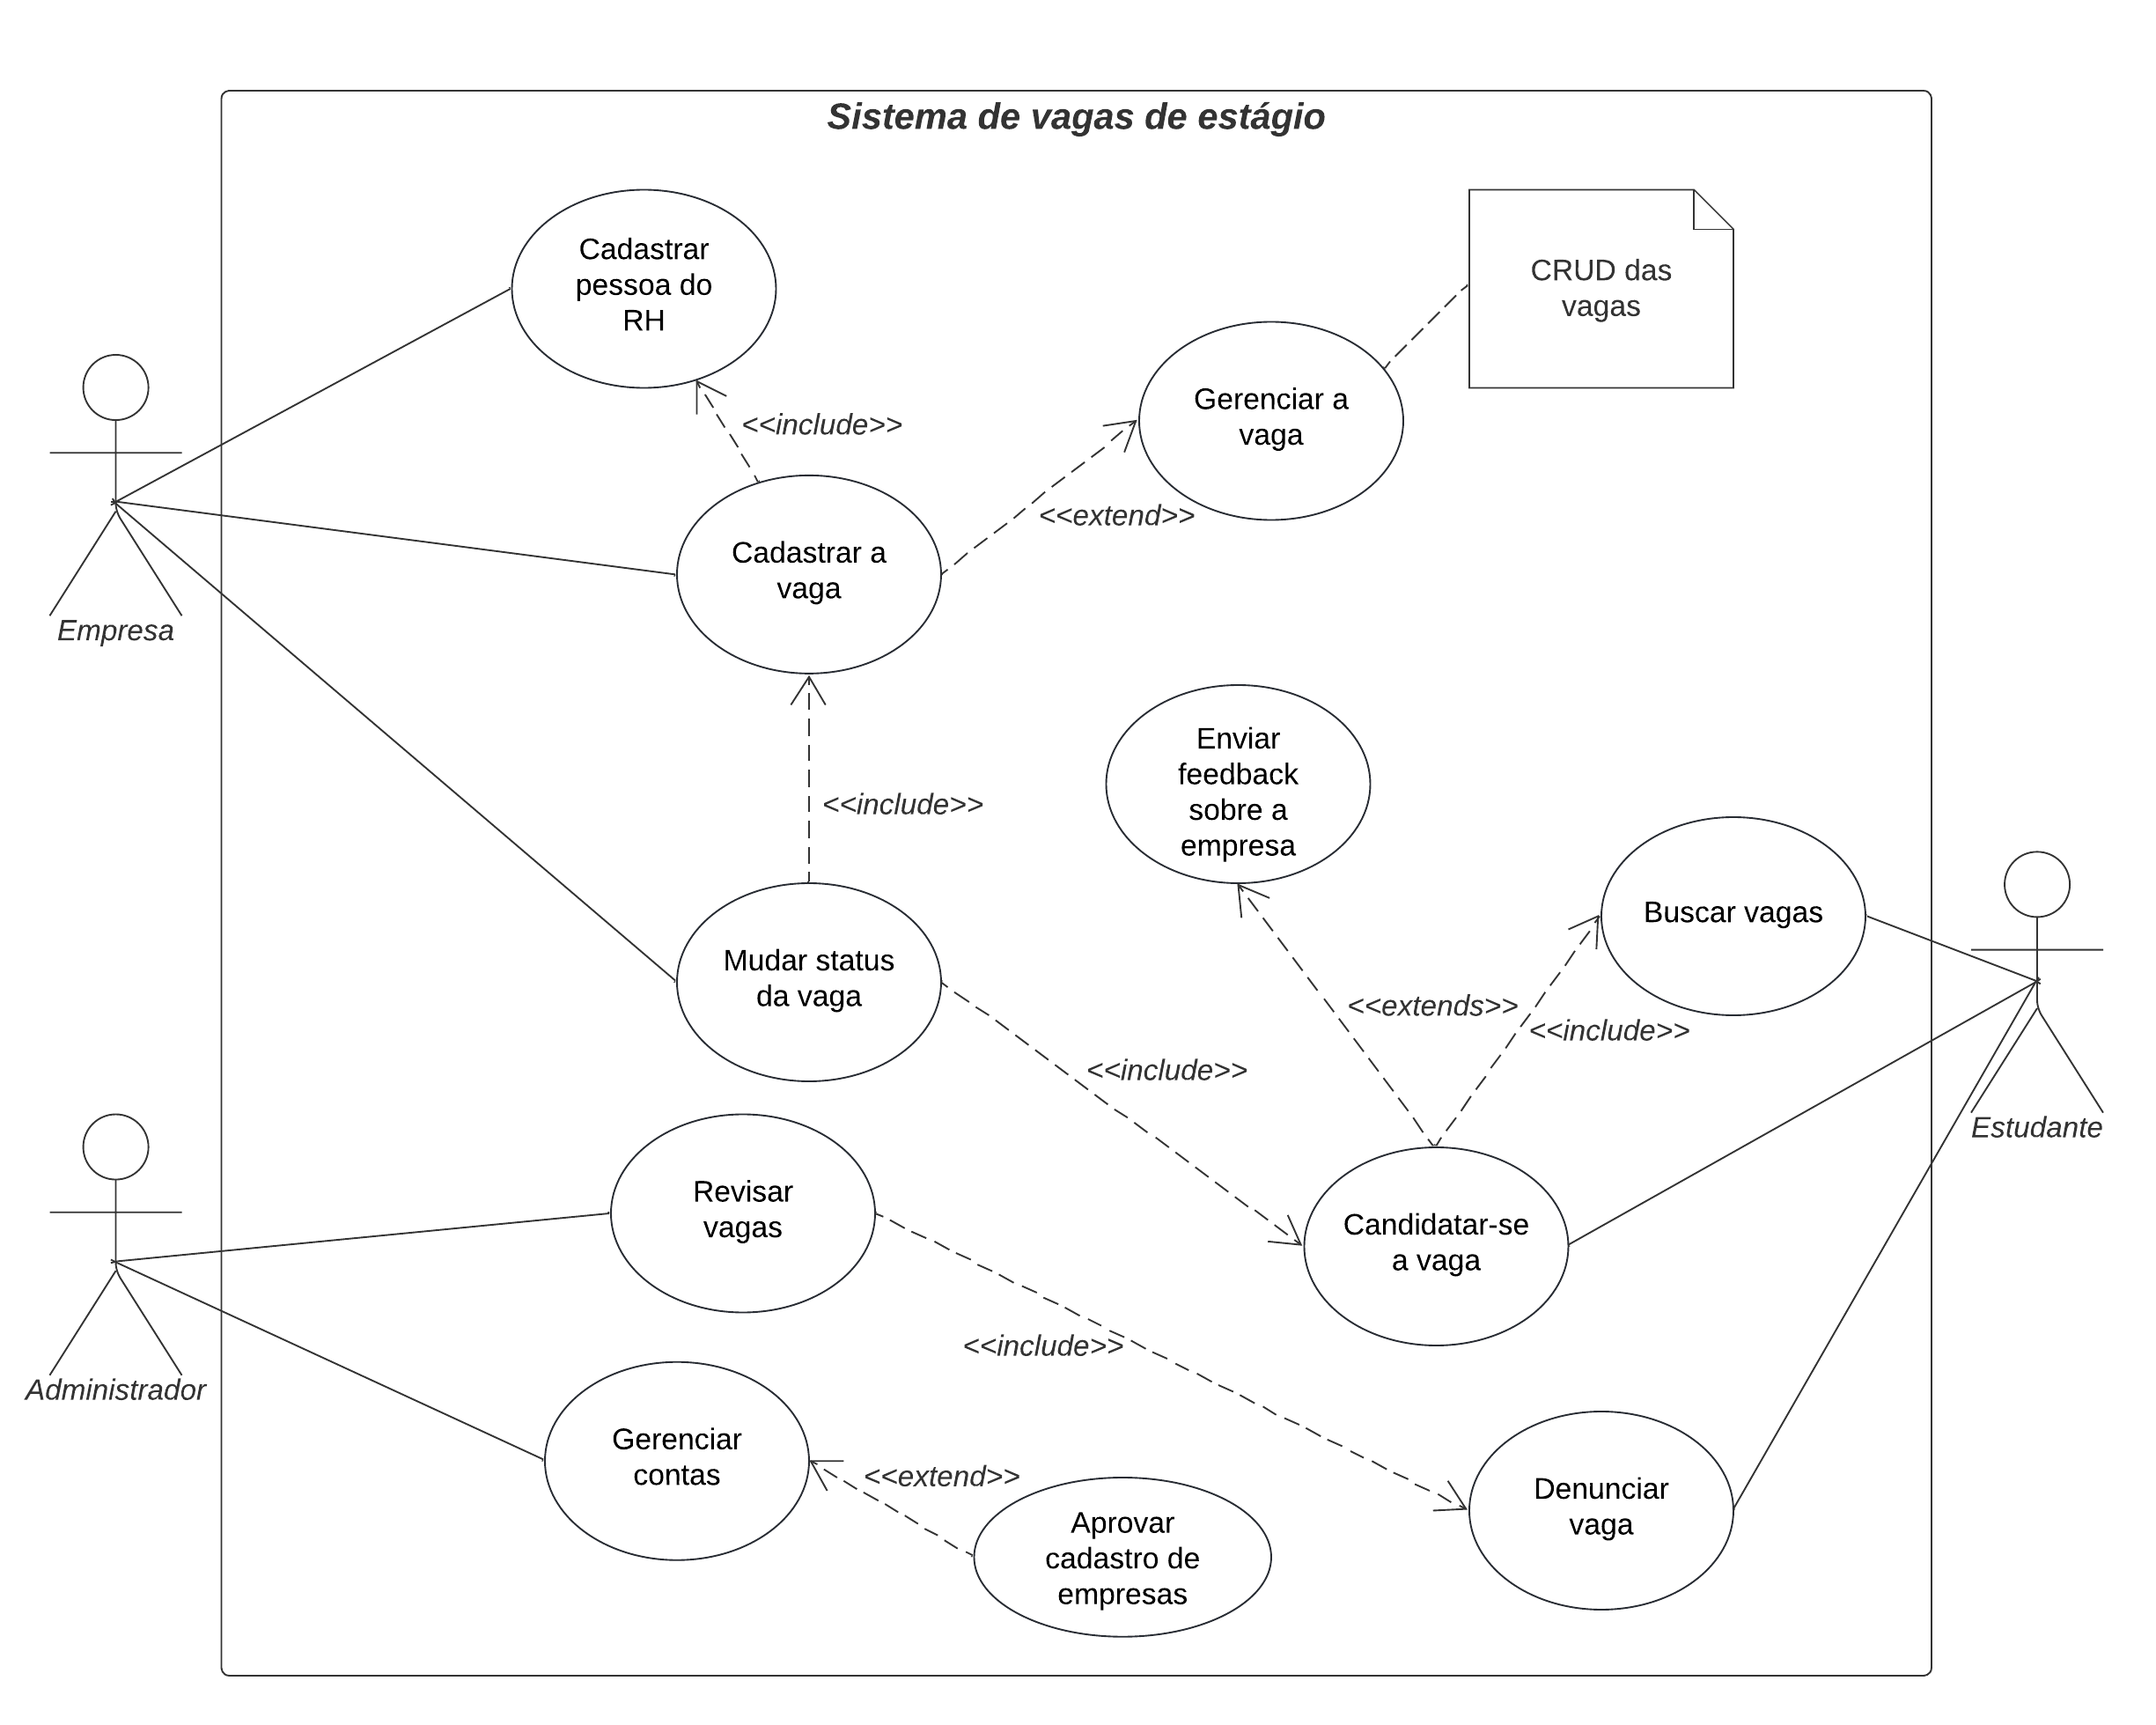
\includegraphics[width=0.8\textwidth]{../imagens/caso-de-uso-todos.png} 
	\fonte{Os autores}
\end{figure}

\subsection{Fases de entrega}

Nessa seção são expostas quais funcionalidades do sistema foram e serão desenvolvidas, tendo em vista as principais fases de entrega da disciplina, sendo elas a \ac{poc}, o \ac{mvp} e a Entrega Final.

\subsubsection{Prova de Conceito (POC)} \label{entrega-poc}

Na fase de \ac{poc}, foram entregues as funcionalidades mais básicas do nosso software. Dentre elas, o cadastro de estudantes via \ac{sso} da \textit{Google}, onde é explicado o processo no site possibilitando a criação de uma conta com informações básicas, necessárias apenas para o funcionamento padrão do sistema, e o cadastro de empresas, que será feito no próprio sistema \emph{EstagiEI}, onde a empresa preenche as informações e passa por uma aprovação da equipe. Além disso, o software permite o \textit{login} desses usuários já cadastrados, onde poderão consultar suas informações básicas.

Ao se cadastrar no sistema, a empresa também poderá registrar uma pessoa do \ac{rh}, que será responsável por gerenciar as vagas daquela organização, e essa pessoa poderá criar novas vagas com informações básicas, apenas para serem visíveis na tela de consulta de vagas. Na parte do estudante, será possível para ele(a), consultar as vagas que existem no sistema através de filtros básicos e internacionalização de linguagem.

\subsubsection{Produto Mínimo Viável (MVP)}

Na entrega do \ac{mvp}, foi incrementado o que já foi desenvolvido durante a \ac{poc} com funcionalidades importantes ao nosso sistema, como a recomendação de vagas ao estudante e edição de perfil. Além disso, foram feitos os testes unitários e validações de segurança, \ac{html}, testes de interface, etc. A fim de garantir que a aplicação esteja em conforme com os requisitos solicitados.

\subsubsection{Entrega Final}

Na entrega final, serão acrescidos no nosso projeto o que já foi feito antes com o restante das funcionalidades, tais como a possibilidade do estudante denunciar uma vaga por não ser coerente com a proposta da nossa aplicação, que é ser um sistema que possua vagas de estágio coerentes com a realidade de um estagiário; recomendação de candidatos para empresas; opção de contato com o candidato via \textit{Whatsapp}; \textit{dashboard} de vagas para a empresa; histórico de vagas para os estudantes; mudança de \textit{status} das vagas por parte da empresa; \textit{feedback} de empresas após o processo seletivo; e acessibilidade com o \gls{vlibras}.